\documentclass{article}
\usepackage{blindtext}
\usepackage[T1]{fontenc}
\usepackage[polish]{babel}
\usepackage[utf8]{inputenc}
\usepackage{graphicx}
\title{Projekt zespołowy - Aplikacja webowa ułatwiająca pracę serwisu komputerowego}
\author{Paweł Pyciński }
\date{16 Maj 2022}

\begin{document}

\maketitle

\section{Opis zasobów domeny biznesowej}
\subsection{Jakie funkcje powinno wykonywać tworzone oprogramowaie?}
\begin{itemize}
    \item możliwość zgłoszenia naprawy
    \item możliowść monitorowania statusu naprawy
    \item wycena kosztów na podstawie wpisanych usług i podzespołów
    \item dodawanie klientów
    \item utworzenie kont klientów*
\end{itemize}


\subsection{Ograniczenia przepisowe}
\begin{itemize}
    \item ze względu na RODO dane użytkowników powinny być przechowywane w bezpieczny i zabezpieczony sposób tak aby nie widzieli ich nawzajem
    \item przy cenach za usługę należy naliczyć odpowiedni podatek
\end{itemize}

\subsection{Opis warstwy technicznej}
\begin{itemize}
    \item konieczne będzie utworzenie odpowiedniej bazy danych do przechowywania danych klientów / części.
    \item pracownicy:
    \begin{enumerate}
        \item prezes (superuser)
        \item sprzedawca lub doradca lub kasjer
        \item serwisant
    \end{enumerate}
    \item Najczęściej będzie dodawane zlecenie naprawy
    \newpage
    \item użytkowany sprzęt w firmie:
    \begin{enumerate}
        \item komputery z windows 10
        \item terminal plikowy NAS
        \item router światłowodowy (szybki dostęp do internetu)
    \end{enumerate}
    \item lokalizacja firmy: Dowolna
\end{itemize}


\section{Wymagania programu opracowane na podstawie opisu domeny}
\subsection{Wymagania funkcjonalne}
\begin{enumerate}
    \item \textbf{\#MUSTx001} zgłoszenia naprawy
    \item \textbf{\#MUSTx002} monitorowanie statusu naprawy
    \item \textbf{\#MUSTx003} wycena kosztów na podstawie wpisanych usług i podzespołów
    \item \textbf{\#MUSTx004} dodawanie klientów
    \item \textbf{\#MUSTx005} dodawanie do cen odpowiedniego podatku
    \item \textbf{\#SHOULDx006} zakładanie kont klienckich
\end{enumerate}
\subsection{wymagania niefunkcjonalne}
\begin{enumerate}
    \item zgodność: system windows 8.1 lub nowszy
    \item konieczne zasoby:
    \begin{itemize}
        \item przeglądarka internetowa obsługująca wszystkie standardy na dzień 12.03.2021.
        \item dostęp do wewnętrznej sieci firmy
    \end{itemize}
    \item ograniczenia czasowe:
    \begin{itemize}
        \item wyszukiwanie danych aplikacja powinna realizować w pesymistycznym czasie $O(n^2)$
        \item projekt wykonany i oddany do końca semestru
    \end{itemize}
    \item bezpieczeństwo:
    \begin{itemize}
        \item użytkownicy nie powinni widzieć cudzych danych ani cudzego sprzętu (RODO)
        \item zmiana statusu naprawy jest możliwa tylko przez serwisanta
    \end{itemize}
\end{enumerate}
\section{Opis domeny biznesowej - przypadki użycia}
\subsection{Przypadek użycia 1: zgłoszenie naprawy w serwisie}
\subsubsection{Opis przypadku}
Przypadek użycia zaczyna się gdy klient chce zgłosić naprawę, przychodzi do serwisu, przynosi sprzęt i zleca naprawę. Kończy się w momencie gdy zgłoszenie jest złożone w systemie.
\subsubsection{Aktorzy}
\begin{itemize}
    \item Doradca sprzedaży - osoba przyjmująca zgłoszenie w serwisie.
    \item Klient - osoba zgłaszająca, przychodzi ze sprzętem do naprawy.
    \item Serwisant - pracowik zaplecza napraw
\end{itemize}
\subsubsection{Warunki początkowe}
Aby rozpocząć przyjęcie zamówienia serwis musi być otwarty, serwer na którym jest postawiona aplikacja powinien być włączony.
Klient zgłaszający musi być w bazie danych klientów.
\subsubsection{Wykonywane czynności przez użytkownika i odpowiedzi systemu}
\begin{enumerate}
    \item doradca sprzedaży loguje się na swoje konto do systemu.
    \item system weryfikuje dane logowania, jeśli są poprawne udziela dostępu do panelu sprzedawcy.
    \item sprzedawca odbiera od klienta sprzęt, znajduje tabliczkę znamionową, wybiera z panelu opcję \textbf{Dodaj zgłoszenie naprawy}.
    \item system w odpowiedzi otwiera formularz umożliwiający dodanie danych sprzętu, usterek.
    \item sprzedawca uzupełnia pola w formularzu. Po zakończeniu, naciska przycisk \textbf{Dodaj zgłoszenie}.
    \item system przetwarza zapytanie i dodaje je do bazy i przekazuje powiadomienie o nowym sprzęcie w serwisie serwisantowi. Wyświetla szacunkowy koszt naprawy.
    \item sprzedawca oznajmia klietowi że sprzęt został dodał dodany oraz podaje szacunkowy koszt usługi.
\end{enumerate}
\subsubsection{Przerwania, możliwe awarie}
\begin{enumerate}
    \item Może wystąpić problem z komputerem pracownika serwisu lub przerwa w dostawie prądu, może on niespodziewanie wyłączyć się lub uruchomić ponownie. Może to wystąpić na każdym etapie realizowania zamówienia i jest niezależna od aplikacji.
    \item Serwer na którym jest postawiona aplikacja może ulec awarii, zawieszeniu lub trwałemu uszkodzeniu fizycznemu spowodowane na przykład nierozawżnym sprzątaniem lokalu. Błąd nastąpi w punkcie 1 basic flow, serwer nie odpowie na żądanie doradcy.
    \item Doradca sprzedaży może zapomieć swojego hasła do systemu, wtedy wystąpi błąd w punkcie 2 basic flow co pociągnie za sobą brak możliwości dodania sprzętu.
    \item Możliwe jest także przeciążenie serwera gdy będzie używać go więcej użytkowników niż jest to określone w specyfikacji technicznej. Awaria nastąpi w punkcie 1 basic flow.
    \item Jeśli doradca sprzedaży będzie próbował dodać większą liczbę zgłoszeń niż maksymalna dozowlona w wymaganiach niefunkcjonalnych, system nie pozwoli aby doszło do przepełnienia magazynu danych i ich utraty pociągając za sobą brak możliwości dodania zgłosznia. Błąd nastąpi w 6 punkcie basic flow.
    \item W przypadku dodania złej usługi przez doradcę sprzedaży (takiej której nie ma w systemie) na przykład mycie samochodu. Apilkacja nie pozwoli na dodanie takiego zgłoszenia do bazy, błąd nastąpi w 6 puncie basic flow.
\end{enumerate}
\subsubsection{Warunki końcowe}
System po poprawnym dodaniu sprzętu do bazy wyświetli komunikat informujący użytkownika że jego zgłoszenie zostało poprawnie przyjęte do systemu.
\subsubsection{Wymagania dodatkowe}
\begin{itemize}
    \item Aby aplikacja webowa wyświetlała poprawnie wszystkie grafiki, panele oraz formularze konieczne będzie posiadanie przeglądarki interetowej obsługującej najnowsze protokoły i standardy na dzień 19.03.2021.
    \item Należy dobrze dobrać miejsce przechowywania serwera aby nie uległ on fizyczej awarii.
    \item W przypadku braku tabliczki znamionowej na urządzeniu należy sprawdzić model sprzętu pod pokrywą obudowy gdyż tam również często są umieszczane tabliczki znamionowe.
    \item Przy implementacji należy pamiętać o uwzględnieniu limitu zgłoszeń aby nie doprowadzić do awarii systemu.
\end{itemize}
\subsection{Przypadek użycia 2: sprawdzenie statusu naprawy}
\subsubsection{Opis przypadku}
Przypadek zaczyna się w momencie gdy klient przychdzi do serwisu i chce dowiedzieć się na jakim etapie jest naprawa jego sprzętu.
\subsubsection{Aktorzy}
\begin{itemize}
    \item Doradca sprzedaży - osoba przyjmująca zgłoszenie w serwisie.
    \item Klient - osoba zgłaszająca, przychodzi ze sprzętem do naprawy.
    \item Serwisant - pracowik zaplecza napraw.
\end{itemize}
\subsubsection{Warunki początkowe}
Aby rozpocząć sprawdzanie statusu zamówienia serwis musi być otwarty, serwer na którym jest postawiona aplikacja powinien być włączony.
\subsubsection{Wykonywane czynności przez użytkownika i odpowiedzi systemu}
\begin{enumerate}
    \item doradca sprzedaży loguje się na swoje konto do systemu.
    \item system weryfikuje dane logowania, jeśli są poprawne udziela dostępu do panelu sprzedawcy.
    \item sprzedawca prosi klienta o numer zgłoszenia, wybiera zakładkę \textbf{Naprawy}, po numerze naprawy wyszukuje zlecenie.
    \item serwer przetwarza zapytanie, zwraca wiersz lub wiersze o pasującym numerze.
    \item sprzewaca oznajumje klietowi jaki jest status naprawy sprawdzając po kolumnie status naprawy.
\end{enumerate}
\subsubsection{Przerwania, możliwe awarie}
\begin{enumerate}
    \item Może wystąpić problem z komputerem pracownika serwisu lub przerwa w dostawie prądu, może on niespodziewanie wyłączyć się lub uruchomić ponownie. Może to wystąpić na każdym etapie realizowania zamówienia i jest niezależna od aplikacji.
    \item Serwer na którym jest postawiona aplikacja może ulec awarii, zawieszeniu lub trwałemu uszkodzeniu fizycznemu spowodowane na przykład nierozawżnym sprzątaniem lokalu. Błąd nastąpi w punkcie 1 basic flow, serwer nie odpowie na żądanie doradcy.
    \item Doradca sprzedaży może zapomieć swojego hasła do systemu, wtedy wystąpi błąd w punkcie 2 basic flow co pociągnie za sobą brak możliwości dodania sprzętu.
    \item Możliwe jest także przeciążenie serwera gdy będzie używać go więcej użytkowników niż jest to określone w specyfikacji technicznej. Awaria nastąpi w punkcie 1 basic flow.
    \item Sprzedawca wpisze niepoprawny numer zgłoszenia, spowodany np literówką, system nie znajdzie zgłoszenia błąd w basic flow 3.
\end{enumerate}
\subsubsection{Warunki końcowe}
System wyświetla wiersz z bazy dotyczący danego zgłosznia naprawy.
\subsubsection{Wymagania dodatkowe}
\begin{itemize}
    \item Aby aplikacja webowa wyświetlała poprawnie wszystkie grafiki, panele oraz formularze konieczne będzie posiadanie przeglądarki interetowej obsługującej najnowsze protokoły i standardy na dzień 19.03.2021.
    \item Należy dobrze dobrać miejsce przechowywania serwera aby nie uległ on fizyczej awarii.
    \item Należy uważnie przepisywać numer zgłoszenia.
    \item Przy implemetacji warto także usunąć niektóre kolumny aby nie było nadmiaru informacji typu, kto naprawia, jakie części itp.
\end{itemize}
\subsection{Przypadek użycia 3: Wycena naprawy}
\subsubsection{Opis przypadku}
Przypadek zaczyna się w momencie gdy klient przychdzi do serwisu i chce dowiedzieć się jakie będą koszta naprawy sprzętu.
\subsubsection{Aktorzy}
\begin{itemize}
    \item Doradca sprzedaży - osoba przyjmująca zgłoszenie w serwisie.
    \item Klient - osoba zgłaszająca, przychodzi ze sprzętem do naprawy.
    \item Serwisant - pracowik zaplecza napraw.
\end{itemize}
\subsubsection{Warunki początkowe}
Aby rozpocząć wycenę serwis musi być otwarty, serwer na którym jest postawiona aplikacja powinien być włączony.
\subsubsection{Wykonywane czynności przez użytkownika i odpowiedzi systemu}
\begin{enumerate}
    \item doradca sprzedaży loguje się na swoje konto do systemu.
    \item system weryfikuje dane logowania, jeśli są poprawne udziela dostępu do panelu sprzedawcy.
    \item sprzedawca odbiera od klienta sprzęt, znajduje tabliczkę znamionową, wybiera z panelu opcję \textbf{Wyceń naprawe}.
    \item system w odpowiedzi otwiera formularz umożliwiający dodanie danych sprzętu oraz usterki.
    \item sprzedawca uzupełnia pola w formularzu. Po zakończeniu, naciska przycisk \textbf{Podaj wycenę}.
    \item system przetwarza zapytanie. Wyświetla szacunkowy koszt naprawy.
    \item sprzedawca podaje szacunkowy koszt usługi.
\end{enumerate}
\subsubsection{Przerwania, możliwe awarie}
\begin{enumerate}
    \item Może wystąpić problem z komputerem pracownika serwisu lub przerwa w dostawie prądu, może on niespodziewanie wyłączyć się lub uruchomić ponownie. Może to wystąpić na każdym etapie realizowania zamówienia i jest niezależna od aplikacji.
    \item Serwer na którym jest postawiona aplikacja może ulec awarii, zawieszeniu lub trwałemu uszkodzeniu fizycznemu spowodowane na przykład nierozawżnym sprzątaniem lokalu. Błąd nastąpi w punkcie 1 basic flow, serwer nie odpowie na żądanie doradcy.
    \item Doradca sprzedaży może zapomieć swojego hasła do systemu, wtedy wystąpi błąd w punkcie 2 basic flow co pociągnie za sobą brak możliwości dodania sprzętu.
    \item Możliwe jest także przeciążenie serwera gdy będzie używać go więcej użytkowników niż jest to określone w specyfikacji technicznej. Awaria nastąpi w punkcie 1 basic flow.
    \item W przypadku dodania złej usługi przez doradcę sprzedaży (takiej której nie ma w systemie) na przykład. mycie samochodu. Apilkacja nie pozwoli na dodanie takiego zgłoszenia do bazy, błąd nastąpi w 6 puncie basic flow.
\end{enumerate}
\subsubsection{Warunki końcowe}
System wyświetla wiersz z bazy dotyczący danego zgłosznia naprawy.
\subsubsection{Wymagania dodatkowe}
\begin{itemize}
    \item Aby aplikacja webowa wyświetlała poprawnie wszystkie grafiki, panele oraz formularze konieczne będzie posiadanie przeglądarki interetowej obsługującej najnowsze protokoły i standardy na dzień 19.03.2021.
    \item Należy dobrze dobrać miejsce przechowywania serwera aby nie uległ on fizyczej awarii.
    \item Przy implemetacji warto uwzględnić informację o tym, że jakiejś części nie ma na stanie.
\end{itemize}
\subsection{Przypadek użycia 4: Dodanie klieta}
\subsubsection{Opis przypadku}
Przypadek zaczyna się w momencie gdy klient jest w serwisie, i nie ma go w bazie. Kończy gdy klient zostanie dodany do systemu.
\subsubsection{Aktorzy}
\begin{itemize}
    \item Doradca sprzedaży - osoba przyjmująca zgłoszenie w serwisie.
    \item Klient - osoba zgłaszająca, przychodzi ze sprzętem do naprawy.
\end{itemize}
\subsubsection{Warunki początkowe}
Aby rozpocząć dodanie klienta serwis musi być otwarty, serwer na którym jest postawiona aplikacja powinien być włączony oraz pracownik serwisu musi być zalogowany do niego
na swoje konto. Klient dodawany do bazy nie może już w niej być.
\subsubsection{Wykonywane czynności przez użytkownika i odpowiedzi systemu}
\begin{enumerate}
    \item doradca sprzedaży klika w zakładkę \textbf{Dodaj klienta}.
    \item serwer przetwarza zapytanie, wyświetla odpowiedni formularz.
    \item sprzedawaca prosi klienta o dane następnie wpisuje je do systemu.
    \item system przetwarza zapytanie, następne wyświetla komunikat o poprawnym dodaniu użytkownika do bazy.
\end{enumerate}
\subsubsection{Przerwania, możliwe awarie}
\begin{enumerate}
    \item Może wystąpić problem z komputerem pracownika serwisu lub przerwa w dostawie prądu, może on niespodziewanie wyłączyć się lub uruchomić ponownie. Może to wystąpić na każdym etapie realizowania zamówienia i jest niezależna od aplikacji.
    \item Serwer na którym jest postawiona aplikacja może ulec awarii, zawieszeniu lub trwałemu uszkodzeniu fizycznemu spowodowane na przykład nierozawżnym sprzątaniem lokalu. Błąd nastąpi w punkcie 1 basic flow, serwer nie odpowie na żądanie doradcy.
    \item Możliwe jest także przeciążenie serwera gdy będzie używać go więcej użytkowników niż jest to określone w specyfikacji technicznej. Awaria nastąpi w punkcie 1 basic flow.
    \item Klient dodawany do bazy już w niej jest, błąd basic flow 4.
\end{enumerate}
\subsubsection{Warunki końcowe}
System wyświetli komunikat o poprawnie dodanym użytkowniku do bazy.
\subsubsection{Wymagania dodatkowe}
\begin{itemize}
    \item Aby aplikacja webowa wyświetlała poprawnie wszystkie grafiki, panele oraz formularze konieczne będzie posiadanie przeglądarki interetowej obsługującej najnowsze protokoły i standardy na dzień 19.03.2021.
    \item Należy dobrze dobrać miejsce przechowywania serwera aby nie uległ on fizyczej awarii.
    \item Przy implemetacji należy sprawdzić czy nie dodajemy drugi raz tej samej osoby.
\end{itemize}
\subsection{Przypadek użycia 5: Dodanie podatków do ceny}
\subsubsection{Opis przypadku}
Przypadek zaczyna się w momencie pobrania ceny z bazy, kończy gdy wyliczona cena zostanie wpisana do rubyki w sekcji koszty naprawy.
\subsubsection{Aktorzy}
\begin{itemize}
    \item Doradca sprzedaży - osoba przyjmująca zgłoszenie w serwisie.
\end{itemize}
\subsubsection{Warunki początkowe}
Aby rozpocząć dodanie klienta serwis musi być otwarty, serwer na którym jest postawiona aplikacja powinien być włączony oraz pracownik serwisu musi być zalogowany do niego
na swoje konto. Pracownik musi być w trakcie dodawania zgłoszenia, wpisuje nazwy podzespołów koniecznych do naprawy sprzętu.
\subsubsection{Wykonywane czynności przez użytkownika i odpowiedzi systemu}
\begin{enumerate}
    \item doradca sprzedaży wpisuje nazwę części w odpowiednim polu przy dodawaniu lub wycenie zgłoszenia.
    \item system korzystając z tabeli w której zawarte są informacje o aktualnych podatakach oblicza cenę z vat i dopisuje ją do części / usługi.
\end{enumerate}
\subsubsection{Przerwania, możliwe awarie}
\begin{enumerate}
    \item Może wystąpić problem z komputerem pracownika serwisu lub przerwa w dostawie prądu, może on niespodziewanie wyłączyć się lub uruchomić ponownie. Może to wystąpić na każdym etapie realizowania zamówienia i jest niezależna od aplikacji.
    \item Serwer na którym jest postawiona aplikacja może ulec awarii, zawieszeniu lub trwałemu uszkodzeniu fizycznemu spowodowane na przykład nierozawżnym sprzątaniem lokalu. Błąd nastąpi w punkcie 1 basic flow, serwer nie odpowie na żądanie doradcy.
    \item Możliwe jest także przeciążenie serwera gdy będzie używać go więcej użytkowników niż jest to określone w specyfikacji technicznej. Awaria nastąpi w punkcie 1 basic flow.
    \item usługa nie znajduje się w bazie, system nie obliczy ceny. Błąd basic flow 2.
\end{enumerate}
\subsubsection{Warunki końcowe}
System doda poporawnie obliczoną cenę do komórki cena.
\subsubsection{Wymagania dodatkowe}
\begin{itemize}
    \item Aby aplikacja webowa wyświetlała poprawnie wszystkie grafiki, panele oraz formularze konieczne będzie posiadanie przeglądarki interetowej obsługującej najnowsze protokoły i standardy na dzień 19.03.2021.
    \item Należy dobrze dobrać miejsce przechowywania serwera aby nie uległ on fizyczej awarii.
    \item Przy implemetacji należy sprawdzić czy usługa jest w serwisie.
\end{itemize}
\subsection{Przypadek użycia 6: Dodanie kont klienckich}
\subsubsection{Opis przypadku}
Przypadek zaczyna się w momencie gdy klient jest w serwisie, i jego dane znajdują się w bazie. Kończy gdy klient dostanie własne konto do logowania w systemie.
\subsubsection{Aktorzy}
\begin{itemize}
    \item Doradca sprzedaży - osoba przyjmująca zgłoszenie w serwisie.
    \item Klient - osoba zgłaszająca, przychodzi ze sprzętem do naprawy.
\end{itemize}
\subsubsection{Warunki początkowe}
Aby rozpocząć dodanie konta klienta serwis musi być otwarty, serwer na którym jest postawiona aplikacja powinien być włączony oraz pracownik serwisu musi być zalogowany do niego
na swoje konto. Ponatdo dane klienta muszą znajdować się w systemie.
\subsubsection{Wykonywane czynności przez użytkownika i odpowiedzi systemu}
\begin{enumerate}
    \item doradca sprzedaży klika w zakładkę \textbf{Dodaj konto}.
    \item serwer przetwarza zapytanie, wyświetla odpowiedni formularz.
    \item sprzedawaca prosi klienta o imię oraz nazwisko, wyszukuje jego dane.
    \item system przetwarza zapytanie, znajduje dane osoby.
    \item sprzedawca wybiera typ konta oraz nadaje mu nazwę oraz hasło.
    \item system zwraca komunikat o poprawnym dodaniu konta do systemu.
\end{enumerate}
\subsubsection{Przerwania, możliwe awarie}
\begin{enumerate}
    \item Może wystąpić problem z komputerem pracownika serwisu lub przerwa w dostawie prądu, może on niespodziewanie wyłączyć się lub uruchomić ponownie. Może to wystąpić na każdym etapie realizowania zamówienia i jest niezależna od aplikacji.
    \item Serwer na którym jest postawiona aplikacja może ulec awarii, zawieszeniu lub trwałemu uszkodzeniu fizycznemu spowodowane na przykład nierozawżnym sprzątaniem lokalu. Błąd nastąpi w punkcie 1 basic flow, serwer nie odpowie na żądanie doradcy.
    \item Możliwe jest także przeciążenie serwera gdy będzie używać go więcej użytkowników niż jest to określone w specyfikacji technicznej. Awaria nastąpi w punkcie 1 basic flow.
    \item Klient którem jest zakładane konto już je posiada. Błąd basic flow 6.
    \item System nie znajdzie danych klienta w bazie. Błąd basic flow 4.
\end{enumerate}
\subsubsection{Warunki końcowe}
System wyświetli komunikat o poprawnie dodanym koncie użytkownika.
\subsubsection{Wymagania dodatkowe}
\begin{itemize}
    \item Aby aplikacja webowa wyświetlała poprawnie wszystkie grafiki, panele oraz formularze konieczne będzie posiadanie przeglądarki interetowej obsługującej najnowsze protokoły i standardy na dzień 19.03.2021.
    \item Należy dobrze dobrać miejsce przechowywania serwera aby nie uległ on fizyczej awarii.
    \item Przy implemetacji należy sprawdzić czy nie dodajemy drugiego konta tej samej osoby oraz czy osoba jest w systemie.
\end{itemize}
\section{Diagramy Uml - graficzne przedstawienie struktur projektu}
\subsection{Diagram sekwencji}
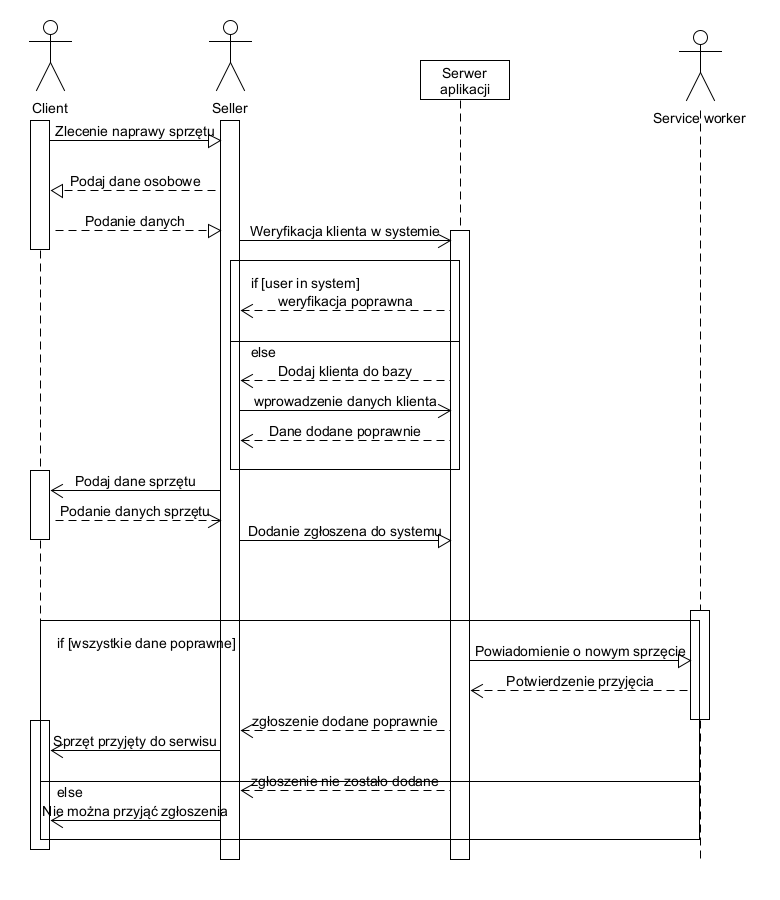
\includegraphics[scale=0.5]{diagrams/sequence_diagram.png}
\subsection{Diagram przypadków użycia}
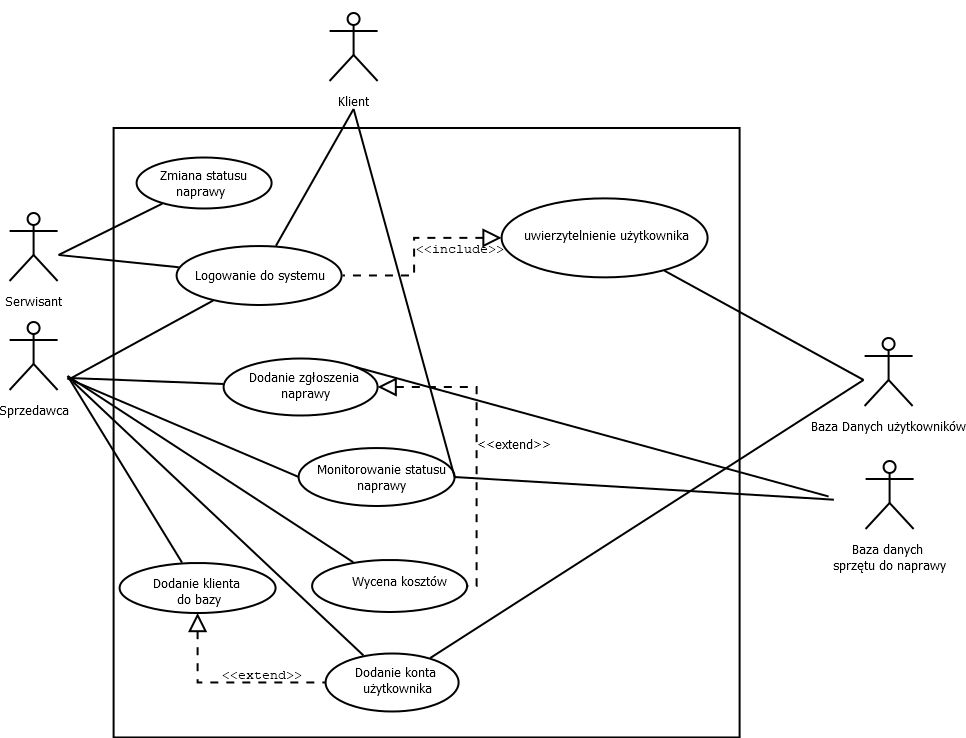
\includegraphics[scale=0.4]{diagrams/use_case_diagram.png}
\end{document}
